In questo esperimento si vuole costruire e studiare un amplificatore \textit{push-pull} in classe B con retroazione e valutare l'effetto della retroazione sulla distorsione di crossover. Il circuito, riportato in Figura \ref{fig:Circuito3}, è lo stesso utilizzato nell' esperienza precedente, l'unica modifica attuata è quella di introdurre una retroazione tra l'uscita e il morsetto invertente dell'operazionale del secondo stadio. Il circuito viene alimentato dalla tensione duale $\pm V_{CC}=\pm 12V$.
\begin{figure}[H]
    \centering
    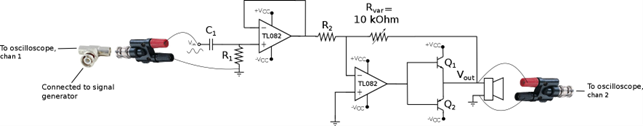
\includegraphics[width=\linewidth]{images/Circuit3.png}
    \caption{Schema circuito}
    \label{fig:Circuito3}
\end{figure}
\subsection{Considerazioni sul circuito}
Attraverso l’implementazione della retroazione si ottiene l’effetto di attenuazione della zona di crossover in uscita, dato che la retroazione è introdotta dopo i transistor, quindi tiene già in considerazione la caduta di tensione sulle giunzioni base-emettitore dei BJT.
\begin{itemize}
    \item Se $V_I=0$ entrambi i transistor sono spenti e $V_0=0$.
    \item Se $V_I > 0.5 V$ $Q_1$ si comporta come un inseguitore di emettitore e $V_O = V_I - V_{beQ1}$, mentre $Q_2$ è spento. 
    \item Se $V_I < -0.5V$ $Q_2$ si comporta come un inseguitore di emettitore e $V_O = V_I + V_{beQ2}$, mentre $Q_1$ è spento.
\end{itemize}
\noindent In questo esperimento è stato scelto l'operazione TL082 tenendo in considerazione il valore elevato dello slew rate dell'integrato. Si riporta in Tabella \ref{tab:slewrate} un semplice confronto con lo slew rate degli operazionali LM741 e LM1458 utilizzati negli esperimenti precedenti.
\begin{table}[H]
    \centering
    \begin{tabular}{|c|c|}
        \hline
        Integrato&Slew rate\\\hline
        TL082&$13\text{ v/}\mu\text{s}$\\\hline
        LM741&$0.5\text{ v/}\mu\text{s}$\\\hline
        LM1458&$0.5\text{ v/}\mu\text{s}$\\\hline
    \end{tabular}
    \caption{Slew rate degli integrati}
    \label{tab:slewrate}
\end{table}
Si preferisce utilizzare operazionali con slew rate elevato in quanto ad alte frequenze uno slew rate troppo basso comporta un'accensione/spegnimento continuo dei transistor, che è quello che si vuole evitare.
\subsection{Assemblaggi e settaggi}
Il generatore di forma d'onda è stato impostato con il seguente segnale:
\begin{itemize}
    \item Forma d'onda: sinusoidale
    \item Ampiezza iniziale: $100mV$ picco-picco
    \item Frequenza: $330Hz$ (nota Mi)
\end{itemize}
\subsection{Procedura di valutazione e risultati}
Dopo l'accensione dell'alimentazione, l'oscilloscopio è stato impostato in modo da visualizzare il segnale di ingresso e il segnale di uscita. Il potenziometro che regola il volume è stato regolato in modo che il segnale di uscita raggiunga un'ampiezza di $1V_{pp}$.\\\\
In Figura \ref{fig:scope_12} si possono vedere le forme d'onda dei segnali di ingresso e uscita
\begin{figure}[H]
    \centering
    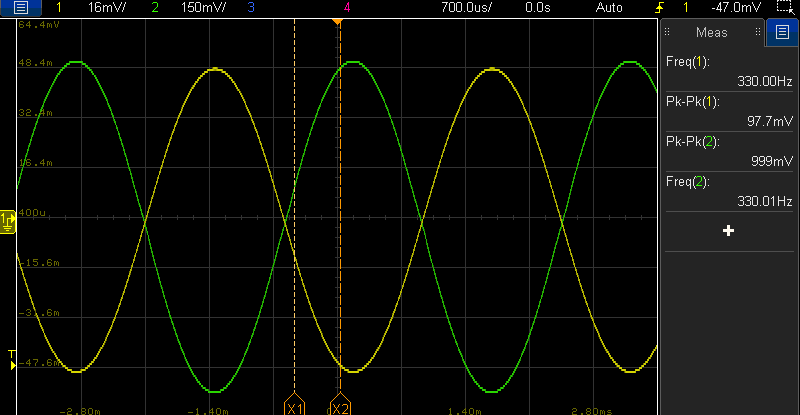
\includegraphics[width=0.7\linewidth]{images/scope_12.png}
    \caption{Segnali di ingresso e uscita dell'amplificatore in classe B con retroazione}
    \label{fig:scope_12}
\end{figure}
Si è proseguito misurando, attraverso i cursori dell’oscilloscopio, l’effetto della distorsione di crossover. Tuttavia, come si vede in Figura \ref{fig:scope_13}, esso è stato completamente eliminato dalla nuova configurazione del circuito.
\begin{figure}[H]
    \centering
    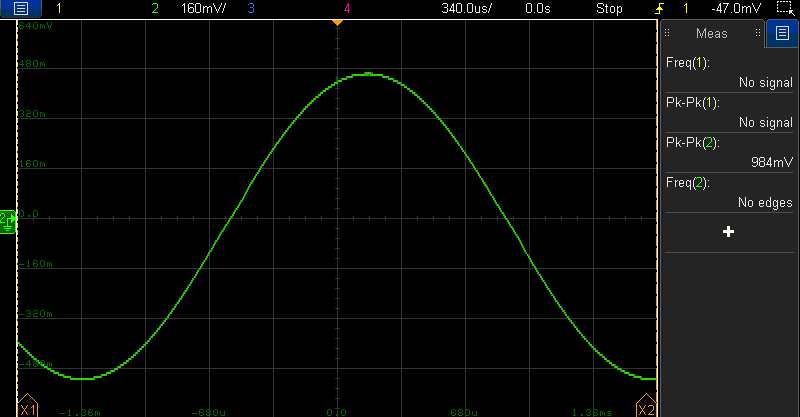
\includegraphics[width=0.7\linewidth]{images/scope_13.png}
    \caption{Dettaglio segnale di uscita}
    \label{fig:scope_13}
\end{figure}
L’unica differenza introdotta nel circuito è il feedback fornito all’amplificatore operazionale, antecedente il push-pull di uscita. Questo tipo di retroazione consente al segnale di ingresso di operare già tenendo conto della caduta di tensione ai capi del transistor, ottenendo così un valore di uscita che consente di bypassare parte della distorsione del crossover dovuta alla zona morta di attivazione del BJT.